\let\negmedspace\undefined
\let\negthickspace\undefined
\documentclass[journal]{IEEEtran}
\usepackage[a5paper, margin=10mm, onecolumn]{geometry}
%\usepackage{lmodern} % Ensure lmodern is loaded for pdflatex
\usepackage{tfrupee} % Include tfrupee package

\setlength{\headheight}{1cm} % Set the height of the header box
\setlength{\headsep}{0mm}  % Set the distance between the header box and the top of the text

\usepackage{gvv-book}
\usepackage{gvv}
\usepackage{cite}
\usepackage{amsmath,amssymb,amsfonts,amsthm}
\usepackage{algorithmic}
\usepackage{graphicx}
\usepackage{textcomp}
\usepackage{xcolor}
\usepackage{txfonts}
\usepackage{listings}
\usepackage{enumitem}
\usepackage{mathtools}
\usepackage{gensymb}
\usepackage{comment}
\usepackage[breaklinks=true]{hyperref}
\usepackage{tkz-euclide} 
\usepackage{listings}
% \usepackage{gvv}                                        
\def\inputGnumericTable{}                                 
\usepackage[latin1]{inputenc}                                
\usepackage{color}                                            
\usepackage{array}                                            
\usepackage{longtable}                                       
\usepackage{calc}                                             
\usepackage{multirow}                                         
\usepackage{hhline}                                           
\usepackage{ifthen}                                           
\usepackage{lscape}
\begin{document}

\bibliographystyle{IEEEtran}
\vspace{3cm}

\title{9.4.9}
\author{EE24BTECH11015 - Dhawal}

% \maketitle
% \newpage
% \bigskip
{\let\newpage\relax\maketitle}

\renewcommand{\thefigure}{\theenumi}
\renewcommand{\thetable}{\theenumi}
\setlength{\intextsep}{10pt} % Space between text and floats

\textbf{Question:}\\
Find the solution of the differential equation $\frac{dy}{dx}=\sin^{-1}{x}$.

\solution{
Solving the given D.E. , we get,
\begin{align}
    \frac{dy}{dx} &= \sin^{-1}{x}
\end{align}

Integrate both sides with respect to $x$:
\begin{align}
y &= \int \sin^{-1}{x} \; dx
\end{align}

Using integration by parts:
\begin{align}
\int u \, dv &= uv - \int v \, du
\end{align}
Let:
\begin{align}
u = \sin^{-1}{x}, \;  dv = dx
\end{align}
Then:
\begin{align}
du = \frac{1}{\sqrt{1-x^2}} \, dx, \; v = x
\end{align}

Substituting into the integration by parts formula:
\begin{align}
\int \sin^{-1}{x} \, dx &= x \sin^{-1}{x} - \int x \frac{1}{\sqrt{1-x^2}} \, dx
\end{align}

For the remaining integral, let $ u = 1 - x^2 $, so $ du = -2x \, dx $:
\begin{align}
\int x \frac{1}{\sqrt{1-x^2}} \, dx &= -\frac{1}{2} \int \frac{1}{\sqrt{u}} \, du \\
&= -\sqrt{u} + C \\
&= -\sqrt{1-x^2} + C
\end{align}


Thus, the solution to the differential equation is:
\begin{align}
y = x \sin^{-1}{x} + \sqrt{1-x^2} + C
\end{align}
\textbf{Computational Solution:}\\
Using a classical definition of derivative, we get,\\
\begin{align}
    f^{\prime}\brak{x} &= \frac{f\brak{x+h}-f\brak{x}}{h}\\
    \implies f\brak{x+h} &= f\brak{x} + h f^{\prime}\brak{x}
\end{align}
By increasing $x$ n each iteration by $h$ and let $C=0$, we are getting $y$ by,
\begin{align}
x_0 &= 0\\
y_0 &= 1\\
h &= 0.01\\
n &= 100
\end{align}
Using Euler Method, we get difference equation,
\begin{align}
y_{n+1} &= y_n + h\frac{dy}{dx}\Big|_{\brak{x_n,y_n}}\\
y_{n+1} &= y_n + h\sin^{-1}{x_n}
\end{align}

\textbf{Using bilinear transfrom:};
\begin{align}
    \frac{dy}{dx} &= \sin^{-1}{x}
\end{align}
Taking Laplase of $\frac{dy}{dx}$ and putting $\sin^{-1}{x}$ as $F\brak{s}$
\begin{align}
    sY\brak{s}&=F\brak{s}\\
    \frac{Y\brak{s}}{F\brak{s}}&=\frac{1}{s}=H\brak{s}
\end{align}
Now, convert it into Z-transform
\begin{align}
    Y\brak{z}&=\frac{h}{2}\frac{1+z^{-1}}{1-z^{-1}}F\brak{z}\\
    Y\brak{z}\brak{1-z^{-1}}&=\frac{h}{2}\brak{1+z^{-1}}F\brak{z}
\end{align}
Applying inverse Z-transform, we get
\begin{align}
    y_{n}-y_{n-1}&=\frac{h}{2}\brak{\sin^{-1}{x_n}+\sin^{-1}{x_{n-1}}}
\end{align}
\begin{figure}[h]
    \centering
    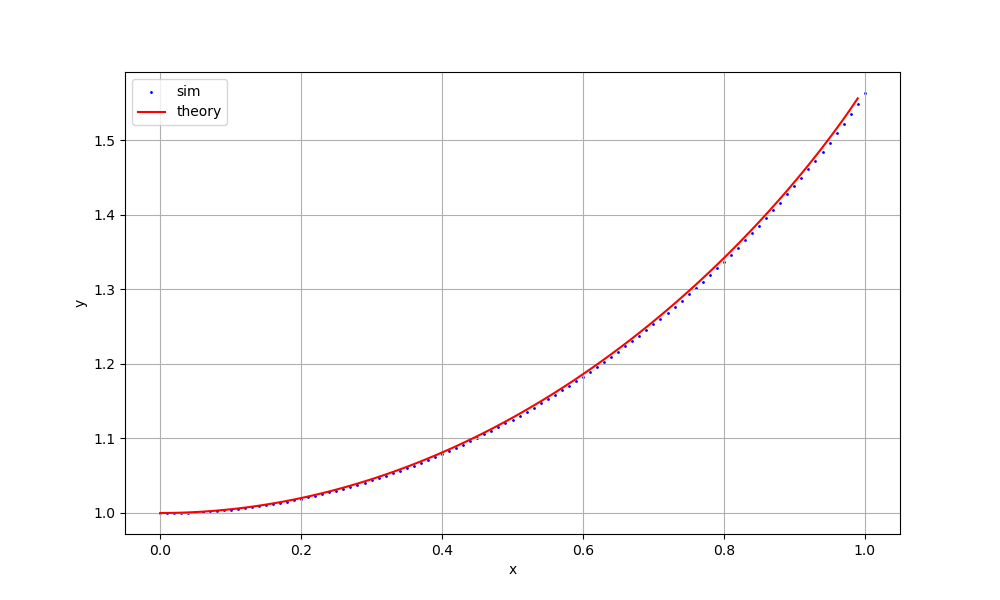
\includegraphics[width=\columnwidth]{figs/Figure_1}
    \caption{Plot of the differential equation }
    \label{fig:Plot}
    \end{figure}

\end{document}
